
\subsection{Mobility}

\textbf{Motivation.} Mobility in chess is a measure of the available moves a player can make in a given position. The idea is that if a player has more available moves, the position is stronger. In \cite{slater:1950} it was shown that there is a strong correlation between a player's mobility and the number of games won. This metric has been used extensively in hand crafted evaluations, and I propose to include this information as features for the neural network. \\

\textbf{Experiment.} There are two ways to go about encoding mobility:

\begin{itemize}
\item \textbf{Bitsets (per piece type):} Provide the exact squares each piece type can move to. Excluding the king, these are $64 * 5 * 2 = 640$ features. The problem with this approach is not the amount of features, but the number of updates to the accumulator per move is very high, which slows down the search.

\begin{figure}[h]
\centering

\begin{tabular}{ccccc}

\raisebox{-7ex}{\chessboard[
    setfen=r5k1/1b1p1ppp/p7/1p1Q4/2p1r3/PP4Pq/BBP2b1P/R4R1K w - - 0 20,
    tinyboard,
    showmover=false,
]}
&

\raisebox{-7ex}{\chessboard[
    tinyboard,
    showmover=false,
    setwhite={ba2,bb2},
    pgfstyle=color,
    opacity=0.8,
    color=blue,
    markfield={b1,c1,c3,d4,e5,f6,g7}
]}

&

\raisebox{-7ex}{\chessboard[
    tinyboard,
    showmover=false,
    addblack={Bb7,Bf2},
    pgfstyle=color,
    opacity=0.8,
    color=blue,
    markfield={c8,c6,d5,a7,b6,c5,d4,e3,e1,g1,g3}
]}

&

\raisebox{-7ex}{\chessboard[
    tinyboard,
    showmover=false,
    setwhite={qd5},
    pgfstyle=color,
    opacity=0.8,
    color=blue,
    markfield={d6,d7,e6,f7,e5,f5,g5,h5,e4,d4,d3,d2,d1,c4,c5,b5,c6,b7}
]}

& $\hdots$

\\

Board &
\makecell{\white White\\\symbishop\ Bishop} &
\makecell{\black Black\\\symbishop\ Bishop} &
\makecell{\white White\\\symqueen\ Queen}

\end{tabular}
\end{figure}


\item \textbf{Counts (per piece type):} Use the number of available moves per piece type as features. This means having a feature for each possible count value, (just) doubling the potential amount of row updates. Further development could bucket this values based on their distribution to reduce some of the updates.

\begin{figure}[H]
\centering
\makebox[\textwidth]{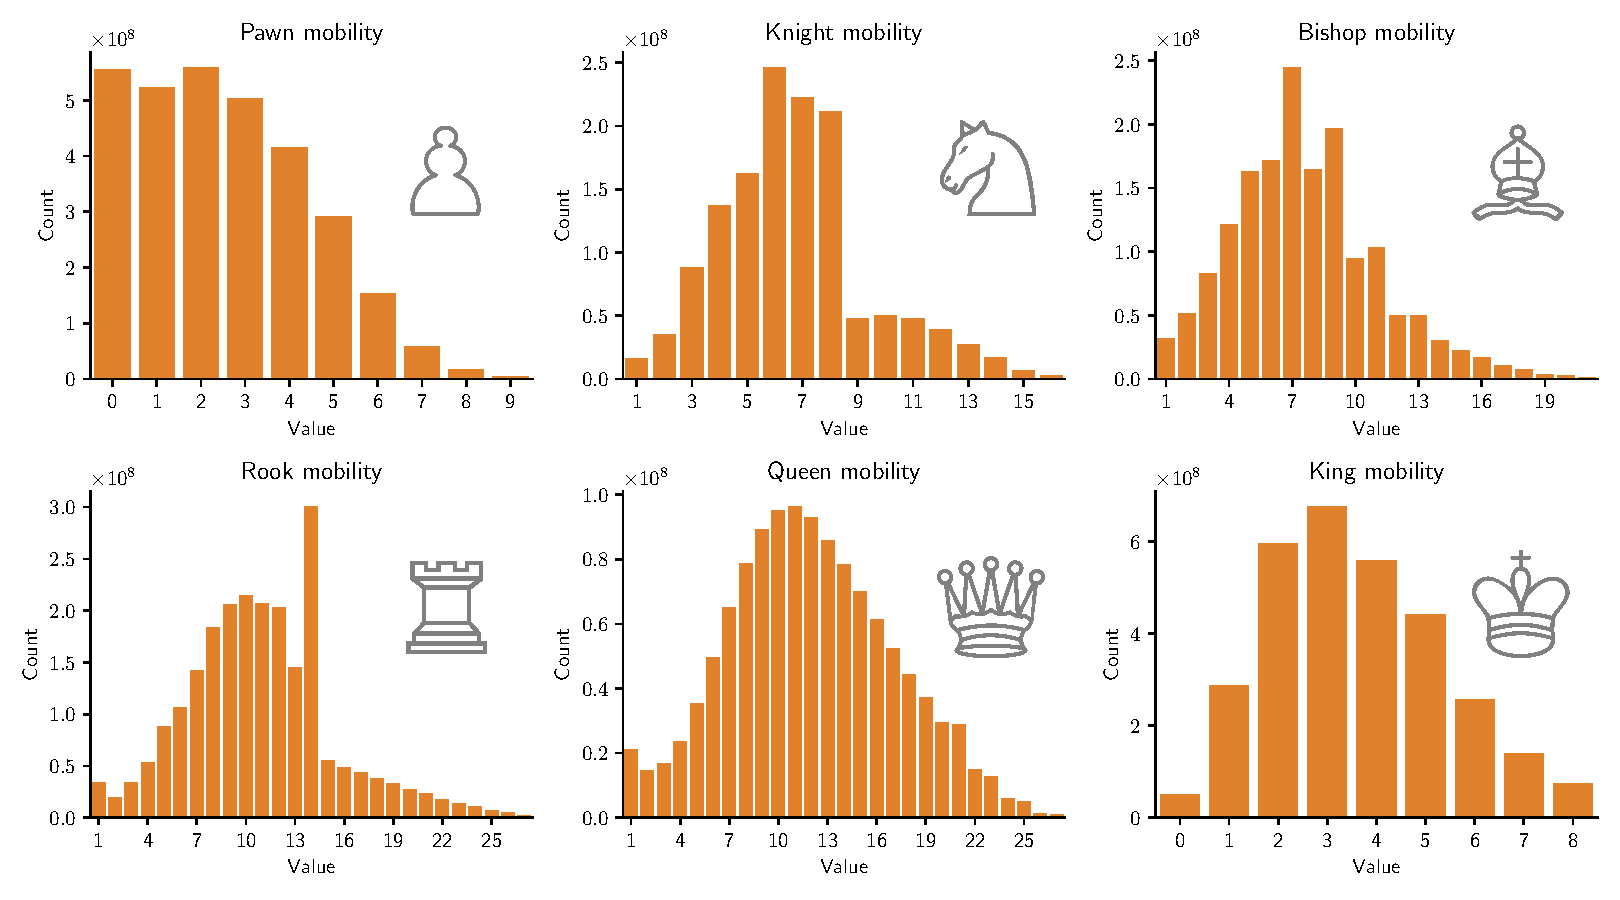
\includegraphics[width=\textwidth]{./dynamic/output/mobility.pdf}}
\caption{Total mobility values for each piece on the board. Computed using 2 billion boards. The value 0 for the Knight, Bishop, Rook and Queen has been excluded from the plot, as it is very common.}
\end{figure}

\end{itemize}

asdasdasd \\

\textbf{Experiment.} asdasd

\textbf{Results.} asdadasdasd
